\documentclass[a4paper,11pt]{article}
\usepackage[utf8]{inputenc}
\usepackage{amsmath}
\usepackage{graphicx}
\usepackage{float}
\usepackage{svg}
\usepackage{hyperref}
\usepackage{geometry}
\usepackage{minted}
\usepackage{titlesec}
\geometry{margin=1in}

\title{You Only Look Once (Yolo)}
\author{BEX Roméo, RIVALDI Tristan, LAMURE Maxence}
\date{24 Septembre 2024}

\begin{document}

\begin{titlepage}

    \begin{minipage}{0.3\linewidth}
     
\includegraphics[width=0.70\textwidth]{../Images/logo_univ.png}   
    \end{minipage}
    \begin{minipage}{0.7\linewidth}
    \LARGE
            \textbf{Université de Montpellier} 
    \end{minipage}
    
    \begin{minipage}{0.3\linewidth}
     
\includegraphics[width=0.60\textwidth]{../Images/logoSSD.png}   
    \end{minipage}
    \begin{minipage}{0.7\linewidth}
    \LARGE
            \textbf{Master 2 Statistiques et Sciences des Données}        
    \end{minipage}
    
    \vspace*{1cm}
    
        \begin{center}
         
            \Huge
    
    \hrulefill
            
            \textbf{You Only Look Once (Yolo)}
    
    \hrulefill

            \vspace{0.5cm}
                
            \large
            \href{https://github.com/RomeoBex/Yolo}{\texttt{https://github.com/RomeoBex/Yolo}}
        
                
                        
            \vspace{2cm}
    
            \Large
            \begin{minipage}[t]{0.4\textwidth}
                 \textbf{Auteurs :}
            \end{minipage}
            \hfill
            \begin{minipage}[t]{0.45\textwidth}
                \raggedleft
                BEX Roméo\\
                RIVALDI Tristan\\ 
                LAMURE Maxence
            \end{minipage}
                
                
            \vspace{9cm}
            \large
            2024 - 2025
                
        \end{center}
    \end{titlepage}

\newpage

\tableofcontents

\newpage

\section*{Introduction}

L'article \textit{You Only Look Once: Unified, Real-Time Object Detection} présente une approche unifiée pour la détection d'objets en temps réel. YOLO reformule la détection d'objets comme un problème de régression directe, de l'image complète aux coordonnées des boîtes englobantes et aux probabilités des classes. Contrairement aux approches classiques, comme R-CNN, qui découpent la tâche en plusieurs étapes (génération de propositions, classification, etc.), YOLO effectue toutes les prédictions en une seule évaluation, ce qui en fait une méthode rapide et efficace. Cette simplicité structurelle permet à YOLO d'atteindre des vitesses inégalées dans le domaine, avec des applications potentielles en conduite autonome, robotique, et surveillance.

\section{Méthodologie}
YOLO suit un pipeline simple mais efficace pour la détection d'objets. Tout d'abord, l'image d'entrée, quelle que soit sa taille initiale, est \textbf{redimensionnée} à une taille fixe de \textbf{448x448 pixels}. Ce redimensionnement est une étape clé, car il garantit que toutes les images traitées par le réseau ont la même dimension, permettant ainsi un traitement cohérent et rapide.

Une fois l'image redimensionnée, elle est ensuite divisée en une grille $S \times S$, où chaque cellule de la grille est responsable de prédire plusieurs boîtes englobantes ($B$) et les scores de confiance associés à ces boîtes. En plus de cela, chaque cellule prédit les probabilités conditionnelles ($C$) pour chaque classe, indiquant la présence d'un objet.

\subsection{Formulation du problème}
La tâche de détection est formulée comme un problème de régression, où le modèle prédit directement les coordonnées de la boîte englobante ainsi que les probabilités des classes. La confiance associée à chaque boîte est donnée par l'équation suivante :

\begin{equation}
\text{Pr(Class}_i | \text{Object}) \times \text{Pr(Object)} \times \text{IOU}_{\text{pred}}^{\text{truth}} = \text{Pr(Class}_i) \times \text{IOU}_{\text{pred}}^{\text{truth}}
\end{equation}

Cette formulation combine la probabilité de présence d'un objet avec l'IoU (intersection over union) entre la boîte prédite et la boîte réelle (ground truth), fournissant une estimation de la qualité de la prédiction.

\subsection{Structure du réseau YOLO}
Le modèle YOLO est basé sur un réseau de convolution profond (CNN), inspiré de GoogLeNet, avec 24 couches convolutionnelles suivies de 2 couches entièrement connectées. Contrairement aux modèles de détection classiques, YOLO traite l'image entière en une seule passe. Voici un schéma représentant l'architecture globale du modèle YOLO (Figure \ref{fig:yolo}).

\begin{figure}[h]
    \centering
    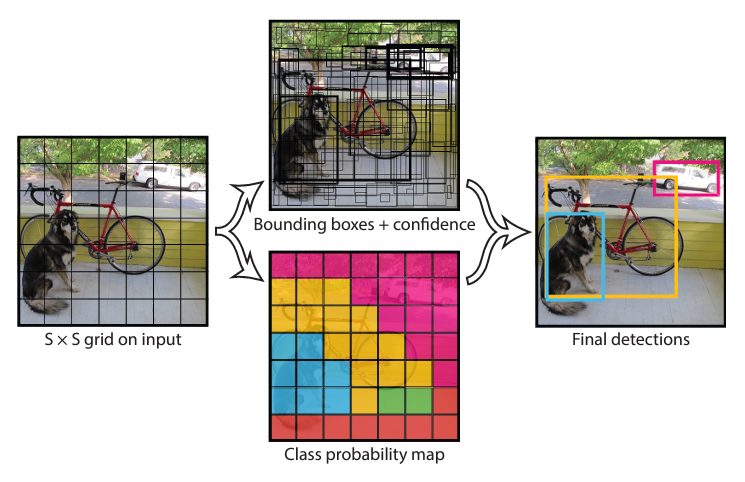
\includegraphics[width=0.8\textwidth]{../Images/yolo_architecture.PNG}
    \caption{Architecture du modèle YOLO. Chaque image est divisée en une grille $S \times S$. Chaque cellule de la grille prédit $B$ boîtes englobantes et $C$ classes.}
    \label{fig:yolo}
\end{figure}

Le réseau prédit un tenseur de taille $S \times S \times (B \times 5 + C)$, où chaque cellule de la grille produit des prédictions pour les coordonnées $(x, y)$, la largeur $w$, la hauteur $h$ et la confiance associée à chaque boîte. Ces prédictions sont directement optimisées par la fonction de perte, que nous décrivons ci-dessous.

\subsection{Fonction de perte}
La fonction de perte utilisée pour entraîner YOLO est cruciale pour la performance du modèle. Elle prend en compte à la fois les erreurs de localisation et de classification. Les prédictions pour les boîtes contenant des objets sont pondérées plus lourdement pour éviter que les cellules sans objets ne dominent la fonction de perte. Pour cela, YOLO utilise deux hyperparamètres, $\lambda_{\text{coord}}$ et $\lambda_{\text{noobj}}$.

\begin{equation}
\lambda_{\text{coord}} \sum_{i=0}^{S^2} \sum_{j=0}^{B} 1^{\text{obj}}_{ij} \left[(x_i - \hat{x}_i)^2 + (y_i - \hat{y}_i)^2\right] + \lambda_{\text{coord}} \sum_{i=0}^{S^2} \sum_{j=0}^{B} 1^{\text{obj}}_{ij} \left[\left(\sqrt{w_i} - \sqrt{\hat{w}_i}\right)^2 + \left(\sqrt{h_i} - \sqrt{\hat{h}_i}\right)^2 \right]
\end{equation}

\begin{equation}
+ \sum_{i=0}^{S^2} \sum_{j=0}^{B} 1^{\text{obj}}_{ij} \left(C_i - \hat{C}_i\right)^2 + \lambda_{\text{noobj}} \sum_{i=0}^{S^2} \sum_{j=0}^{B} 1^{\text{noobj}}_{ij} \left(C_i - \hat{C}_i\right)^2
\end{equation}

Cette fonction de perte complexe permet à YOLO de mieux gérer les situations où les objets sont absents, en réduisant les faux positifs et en minimisant les erreurs de localisation.

\subsection{Prédictions et encodage des boîtes englobantes}
Chaque cellule de la grille $S \times S$ prédit des boîtes englobantes avec des coordonnées $(x, y)$ représentant le centre de la boîte par rapport à la cellule, et $(w, h)$ représentant la largeur et la hauteur relatives à l'image entière. YOLO utilise également l'IoU entre les boîtes prédite et réelle pour ajuster les scores de confiance. La boîte avec le score IoU le plus élevé est sélectionnée pour représenter l'objet.

\section{Comparaison des Méthodes}
YOLO se distingue des méthodes traditionnelles de détection par son architecture simple et unifiée, qui lui permet d'être beaucoup plus rapide tout en ayant une bonne précision. Dans le tableau \ref{tab:performance}, YOLO est comparé à d'autres méthodes de pointe comme Faster R-CNN et Fast R-CNN.

\begin{table}[h]
\centering
\begin{tabular}{|l|c|c|}
\hline
\textbf{Méthode} & \textbf{mAP (\%)} & \textbf{FPS} \\
\hline
Fast R-CNN & 70.0 & 0.5 \\
Faster R-CNN & 73.2 & 7 \\
YOLO & 63.4 & 45 \\
Fast YOLO & 52.7 & 155 \\
\hline
\end{tabular}
\caption{Comparaison des performances de détection sur PASCAL VOC 2007}
\label{tab:performance}
\end{table}

\subsection{Analyse des erreurs}
YOLO présente un profil d'erreur distinct par rapport aux autres systèmes de détection. Comme illustré dans l'article, la majorité des erreurs de YOLO sont des erreurs de localisation. En revanche, il commet moins d'erreurs de fond (background) que Fast R-CNN, qui a tendance à détecter des objets inexistants dans des zones de fond. Cela s'explique par le fait que YOLO voit l'image entière pendant la prédiction, ce qui lui permet d'incorporer des informations contextuelles globales.

\section{Limites et Faiblesses}
Malgré ses avantages en termes de rapidité et de généralisation, YOLO présente certaines limitations :
\begin{itemize}
    \item \textbf{Problèmes de localisation} : YOLO a tendance à commettre des erreurs de localisation, notamment pour les petits objets ou ceux situés près des bords de l'image. Cela est dû aux contraintes imposées par la grille $S \times S$, où chaque cellule ne peut prédire qu'un nombre limité de boîtes.
    \item \textbf{Sensibilité aux petites boîtes} : Les petites erreurs dans les prédictions des boîtes pour des objets de petite taille ont un impact plus important sur l'IoU, ce qui peut affecter négativement les performances globales.
    \item \textbf{Généralisation des aspects visuels} : Bien que YOLO soit performant sur des images naturelles et qu'il généralise bien sur de nouveaux domaines (comme l'art), il peut avoir des difficultés à reconnaître des objets dans des configurations ou proportions inhabituelles.
\end{itemize}

\section{Conclusion}
YOLO propose une solution innovante à la détection d'objets, simplifiant le pipeline complexe des méthodes traditionnelles et permettant une détection en temps réel. Bien qu'il présente des limitations, notamment en termes de localisation précise, sa rapidité et sa capacité à généraliser en font un outil puissant pour des applications nécessitant une détection rapide et robuste. YOLO reste un modèle d'avenir pour des applications en robotique, surveillance, ou réalité augmentée.

\end{document}
